\documentclass[12pt,a4paper]{article}
\usepackage[romanian]{babel}
\usepackage{fontspec}
\setmainfont{TeX Gyre Termes}
\usepackage{geometry,setspace,booktabs,tabularx,array,longtable,xcolor,tikz,xurl,hyperref,pdflscape,enumitem}
\usetikzlibrary{arrows.meta,positioning,calc}
\geometry{top=2.2cm,bottom=2.2cm,left=2.5cm,right=2.5cm}
\onehalfspacing
\definecolor{navy}{HTML}{173A56}\definecolor{redx}{HTML}{8D2930}\definecolor{pale}{HTML}{EDF4F8}
\hypersetup{colorlinks=true,urlcolor=navy,linkcolor=navy}
\setlength{\parindent}{0pt}\setlength{\parskip}{0.45em}
\renewcommand{\arraystretch}{1.22}
\newcommand{\src}[1]{\textsuperscript{[#1]}}
\begin{document}
\begin{center}
{\Large\bfseries Proiect ANI}\\[4pt]
% {\large Cercetare preliminară --- Seminarul 1}\\[4pt]
% {\bfseries Platformă pentru identificarea oportunităților profesionale și optimizarea aplicațiilor}\\[6pt]
{\bfseries Careerly}\\[6pt]
% \textit{Numele proiectului, numărul echipei, membrii și grupa: de completat de echipă}
\end{center}

\section{Problema}
\subsection{Definirea problemei}
\textbf{Enunțul problemei.} Persoanele care caută internshipuri sau locuri de muncă întâmpină dificultăți în identificarea rapidă a ofertelor relevante și în evaluarea compatibilității dintre CV-ul propriu și cerințele fiecărui post; în prezent, caută pe mai multe platforme și își compară sau adaptează manual CV-ul pentru fiecare anunț, ceea ce presupune timp și efort și poate conduce la aplicări slab direcționate.

\textbf{Cine este afectat.} Persoanele aflate în căutarea unui internship sau job, inclusiv candidații aflați la începutul carierei. Accentul pe această categorie este o direcție de cercetare, nu un segment de clienți deja validat.

\textbf{De ce contează.} Problema are două componente legate între ele: (i) descoperirea și filtrarea anunțurilor potrivite; (ii) evaluarea cerințelor și pregătirea unei candidaturi adaptate, fără exagerarea calificărilor. Timpul economisit, claritatea asupra compatibilității și un proces de aplicare mai organizat reprezintă beneficiile urmărite, încă neverificate prin teste cu utilizatori.

\textbf{Date care contextualizează problema.} Potrivit Eurostat, în 2025 rata de angajare a tinerilor absolvenți (20--34 ani, conform definiției statistice) a fost de 83,0\% în UE, față de 72,7\% în România. Indicatorul arată contextul tranziției de la studii la muncă, dar \emph{nu măsoară direct} timpul pierdut căutând joburi sau eficiența CV-urilor. Eurostat raportează și că 63,8\% dintre tinerii de 16--24 de ani din UE au folosit instrumente de AI generativ în 2025, în timp ce în România procentul era 44,1\%; aceste valori indică un context de adoptare tehnologică, nu demonstrează cererea pentru aplicația propusă.

\textbf{Validare necesară.} Interviuri/chestionare cu persoane care aplică efectiv: numărul platformelor consultate, timpul săptămânal petrecut cu căutarea și adaptarea CV-ului, frecvența aplicațiilor, dificultățile principale și disponibilitatea de a plăti.

\vspace{6cm}


% Diagrama de pe pagina următoare diferențiază \textbf{cauzele}, \textbf{problema centrală} și \textbf{efectele}. Legăturile sunt ipoteze cauzale pentru cercetarea preliminară, nu rezultate statistice dovedite.

\begin{landscape}
\subsection{Arborele problemei}
\thispagestyle{plain}
\begin{center}
% {\Large\bfseries Arborele problemei}\\[5pt]
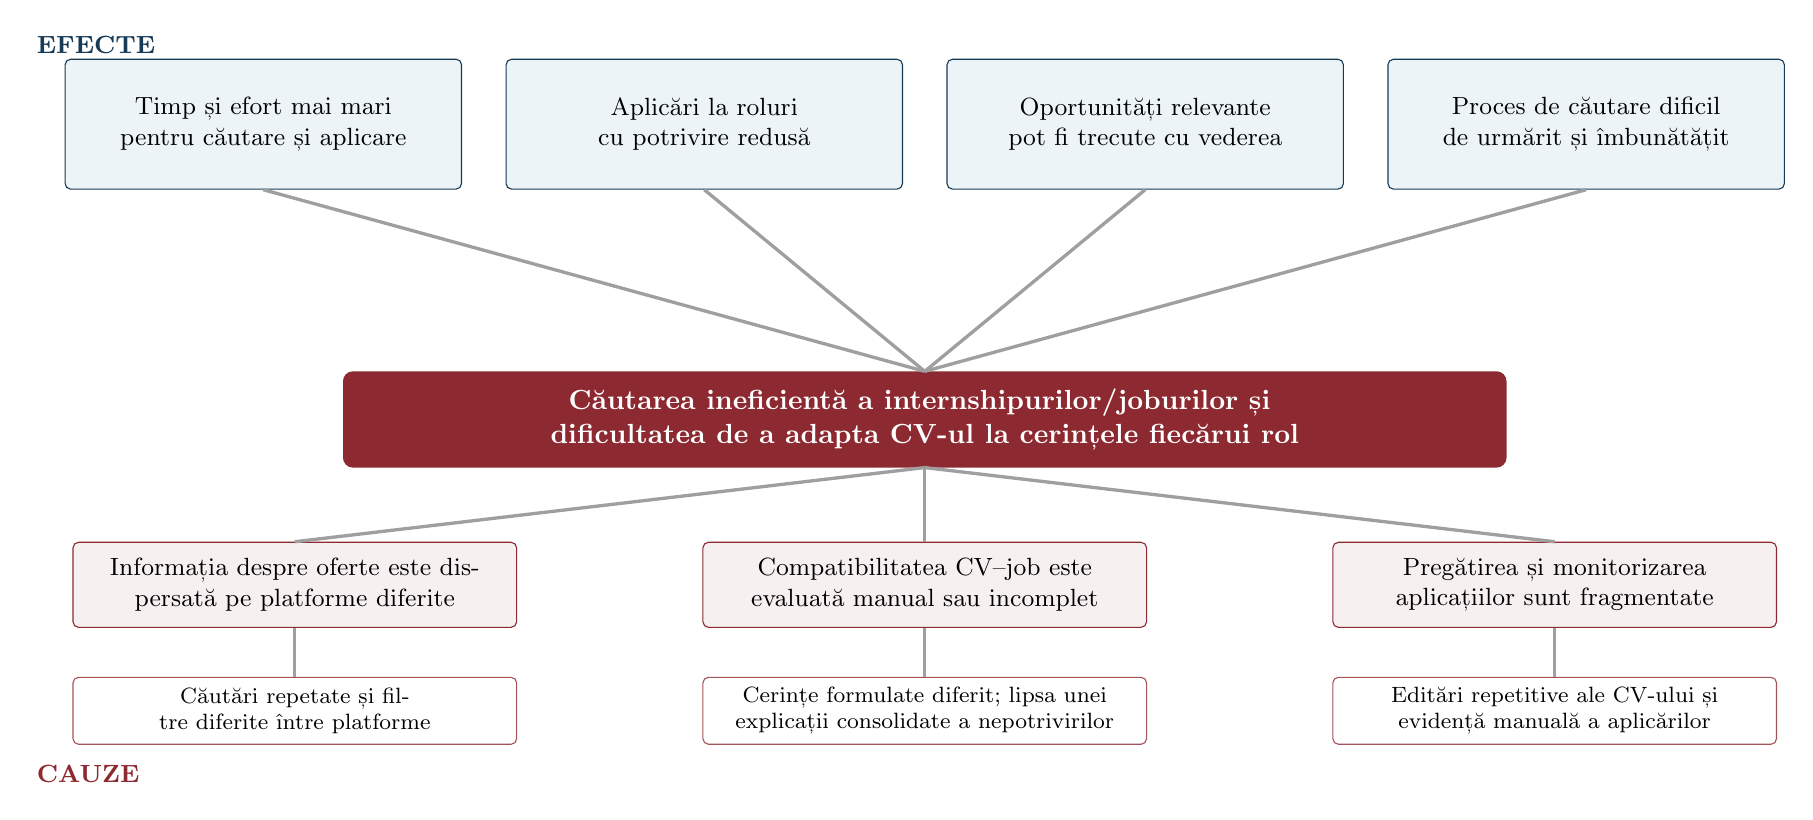
\begin{tikzpicture}[>=Stealth, x=1cm,y=1cm,
 node distance=0.38cm,
 effect/.style={draw=navy,fill=pale,rounded corners=2pt,align=center,font=\small,text width=4.8cm,minimum height=1.65cm},
 cause/.style={draw=redx,fill=redx!7,rounded corners=2pt,align=center,font=\small,text width=5.4cm,minimum height=1.08cm},
 subcause/.style={draw=redx!80,fill=white,rounded corners=2pt,align=center,font=\footnotesize,text width=5.4cm,minimum height=0.85cm},
 center/.style={draw=redx,fill=redx,text=white,very thick,rounded corners=3pt,align=center,font=\bfseries\normalsize,text width=14.5cm,minimum height=1.18cm},
 line/.style={draw=gray!75,very thick}]
\node[effect] (e1) at (-8.4,6.4) {Timp și efort mai mari pentru căutare și aplicare};
\node[effect] (e2) at (-2.8,6.4) {Aplicări la roluri cu potrivire redusă};
\node[effect] (e3) at (2.8,6.4) {Oportunități relevante pot fi trecute cu vederea};
\node[effect] (e4) at (8.4,6.4) {Proces de căutare dificil de urmărit și îmbunătățit};
\node[center] (p) at (0,2.65) {Căutarea ineficientă a internshipurilor/joburilor și \break dificultatea de a adapta CV-ul la cerințele fiecărui rol};
\node[cause] (c1) at (-8,0.55) {Informația despre oferte este dispersată pe platforme diferite};
\node[cause] (c2) at (0,0.55) {Compatibilitatea CV--job este evaluată manual sau incomplet};
\node[cause] (c3) at (8,0.55) {Pregătirea și monitorizarea aplicațiilor sunt fragmentate};
\node[subcause] (s1) at (-8,-1.05) {Căutări repetate și filtre diferite între platforme};
\node[subcause] (s2) at (0,-1.05) {Cerințe formulate diferit; lipsa unei explicații consolidate a nepotrivirilor};
\node[subcause] (s3) at (8,-1.05) {Editări repetitive ale CV-ului și evidență manuală a aplicărilor};
\foreach \e in {e1,e2,e3,e4} {\draw[line] (p.north) -- (\e.south);}
\foreach \c in {c1,c2,c3} {\draw[line] (\c.north) -- (p.south);}
\foreach \a/\b in {s1/c1,s2/c2,s3/c3} {\draw[line] (\a.north) -- (\b.south);}
\node[anchor=west,font=\bfseries\small,text=navy] at (-11.4,7.40) {EFECTE};
\node[anchor=west,font=\bfseries\small,text=redx] at (-11.4,-1.85) {CAUZE};
\end{tikzpicture}
\end{center}
\end{landscape}

\section{Soluții existente}
\subsection{Soluții}
\small
\begin{longtable}{p{2.35cm}p{3.4cm}p{2.05cm}p{5.4cm}}
\toprule
\textbf{Alternativă} & \textbf{Ce oferă} & \textbf{Preț / acces} & \textbf{Limitare relevantă pentru problema noastră}\\\midrule\endhead
Career Ops & Căutare și evaluare de oferte, scor CV--rol, adaptare CV, scrisori, tracker, dashboard TUI. & Open-source; utilizarea modelelor/serviciilor poate implica costuri. & Flux orientat spre terminal și AI CLI; nu reprezintă o interfață grafică web/mobilă pentru utilizatorii fără experiență tehnică.\\
LinkedIn Jobs & Listări de joburi, recomandări, informații privind potrivirea candidat--rol. & Funcții de bază gratuite; unele evaluări avansate sunt Premium. & Este în primul rând o platformă de joburi; avantajul unei experiențe consolidate pe surse multiple trebuie demonstrat, nu presupus.\\
Teal & CV builder, job tracker, comparație cu descrierea postului, sugestii de optimizare. & Gratuit cu limitări; Teal+ 29 USD/30 zile (preț verificat la data consultării). & Are deja UI și matching; diferențierea trebuie să privească întregul flux și uzabilitatea, nu simpla existență a scorului.\\
Jobscan & Analiza CV-ului versus job description; raport de potrivire, cuvinte-cheie și format ATS. & Raport inițial gratuit; acces extins cu plată (preț variabil). & Accent pe evaluarea și optimizarea CV-ului; nu elimină necesitatea unui proces de descoperire a ofertelor în alte locuri.\\
Căutare manuală & Navigare între platforme, comparare personală, editare CV în editor de text. & Fără abonament obligatoriu. & Necesită repetarea sarcinilor și organizarea separată a posturilor și aplicațiilor.\\
\bottomrule
\end{longtable}
\normalsize
\textbf{Soluția de referință pentru SCAMPER: Career Ops.} Alegerea rezultă din apropierea sa funcțională de ideea echipei. Observație importantă: proiectul \emph{are} o interfață TUI (în terminal), nu este lipsit de orice UI.

\subsection{Metoda SCAMPER aplicată pe Career Ops}
\begin{tabularx}{\textwidth}{>{\bfseries}p{2.65cm}X}
% \toprule Componentă & Propunere de schimbare (ipoteză de produs)\\\midrule
\toprule
S --- Substituie & Înlocuirea interacțiunii prin comenzi/terminal cu interacțiuni grafice: formulare, carduri, filtre, progres vizibil.\\
C --- Combină & Integrarea într-un singur traseu a căutării, scorului explicat, adaptării CV-ului și trackerului de aplicări.\\
A --- Adaptează & Preluarea mecanismelor de onboarding ghidat din aplicațiile consumer pentru configurarea profilului și obiectivelor.\\
M --- Modifică & Prezentarea scorului ca evaluare explicabilă, cu cerințe îndeplinite, lipsuri și recomandări concrete, nu ca simplu număr.\\
P --- Pune la altă utilizare & Refolosirea comparației CV--cerințe pentru orientare asupra competențelor de dezvoltat, nu doar pentru un anunț anume.\\
E --- Elimină & Reducerea pașilor tehnici de instalare/configurare și a introducerii repetate a acelorași date, acolo unde este fezabil.\\
R --- Rearanjează & Inversarea fluxului tradițional: întâi filtrarea oportunităților după compatibilitate, apoi investiția de timp în personalizarea aplicației.\\
\bottomrule
\end{tabularx}

\section{Ce aducem nou?}
\textbf{Ideea de produs.} O aplicație cu interfață grafică prietenoasă (platforma web/mobilă urmând a fi decisă) în care utilizatorul își încarcă CV-ul, descoperă oportunități, vede un indicator de compatibilitate explicat și primește propuneri de adaptare a CV-ului bazate exclusiv pe experiențe reale. Utilizatorul verifică și decide ce modifică și unde aplică.

\textbf{Diferențiere propusă.} Nu susținem că scorul de matching sau optimizarea CV-ului sunt invenții proprii: Career Ops, LinkedIn, Teal și Jobscan oferă deja variante ale acestora. Ipoteza noastră de diferențiere este experiența integrată și ghidată pentru candidați care nu doresc să folosească terminalul. Avantajul față de soluțiile care au deja GUI rămâne de testat.

\textbf{Încadrarea inovării după cele trei criterii:}
\begin{itemize}[leftmargin=*,itemsep=0.1em]
\item \textbf{Obiectul inovării:} inovare de produs (aplicație și experiență grafică) și de proces (simplificarea etapelor căutare--evaluare--adaptare--urmărire).
\item \textbf{Amploare:} incrementală; reunim și facem mai accesibile funcții deja disponibile, fără a pretinde descoperirea unei tehnologii radical noi.
\item \textbf{Pentru cine e nouă:} potențial nouă pentru un segment de utilizatori insuficient deservit de interfețele existente; afirmația privind noutatea pentru România sau la nivel mondial \emph{nu poate fi făcută} fără cercetare competitivă suplimentară.
\end{itemize}

\textbf{Fișa de inovare --- evaluare preliminară a echipei (scoruri orientative, de validat):}
\par\medskip
\begin{tabularx}{\textwidth}{p{2.6cm}p{1.15cm}X}
\toprule Criteriu & Scor /5 & Argument\\\midrule
Noutate & 2 & Există deja produse cu potrivire CV--job, recomandări și UI.\\
Diferențiere & 3 & Posibilă prin flux mai simplu; nu există încă teste comparative de uzabilitate.\\
Greu de copiat & 2 & Un UI poate fi reprodus; un avantaj sustenabil ar necesita feedback, date și integrare bună.\\
Tehnologie & 4 & Analiza descrierilor, compararea semantică și generarea asistată sunt centrale pentru propunere.\\
Mărimea problemei & 3 & Datele privind inserția profesională contextualizează piața; amploarea dificultății specifice nu e încă cuantificată.\\
\bottomrule
\end{tabularx}
% \textit{Scorurile sunt judecăți de lucru, nu rezultate ale unui studiu de piață.}

\section{De ce acum?}
\textbf{1. Factor tehnologic.} Instrumentele AI generative pot susține extragerea cerințelor și reformularea asistată a textului. Adoptarea AI generative de către 63,8\% dintre tinerii UE de 16--24 ani în 2025 sugerează o familiaritate în creștere cu această categorie de instrumente; nu dovedește singură disponibilitatea de a utiliza produsul propus.

\textbf{2. Factor social.} Candidații au deja acces la evaluări de potrivire între profil/CV și anunț: LinkedIn descrie explicit acest tip de funcționalitate. Existența practicii arată că un flux de potrivire asistată este deja relevant în oferta platformelor actuale; rămâne de măsurat interesul utilizatorilor pentru o alternativă cu experiență grafică unificată.

\textbf{3. Factor economic și de piață a muncii.} Diferența dintre rata de angajare a absolvenților recenți din România (72,7\%) și media UE (83,0\%) în 2025 motivează cercetarea tranziției către primul job. Nu demonstrează că un instrument de CV-matching ar corecta această diferență, însă justifică explorarea soluțiilor care reduc fricțiunile de căutare.

\textbf{Element transversal.} Disponibilitatea unei baze open-source actuale, Career Ops, facilitează prototiparea și evaluarea unei experiențe grafice, sub rezerva examinării licenței, a arhitecturii și a limitărilor tehnice înainte de reutilizare.

% \section*{Surse și bibliografie}
% \begin{enumerate}[label={[\arabic*]},leftmargin=*,itemsep=0.1em]
% \item Eurostat, \emph{Employment of recent graduates reached 83\% in 2025}, 15.06.2026. \url{https://ec.europa.eu/eurostat/en/web/products-eurostat-news/w/ddn-20260615-1}
% \item Eurostat, \emph{64\% of 16--24-year-olds used AI in 2025}, 10.02.2026. \url{https://ec.europa.eu/eurostat/en/web/products-eurostat-news/w/edn-20260210-1}
% \item Career Ops, repository și README (consultat 16.10.2026). \url{https://github.com/career-ops-hq/career-ops}
% \item LinkedIn Help, \emph{Find how you match up with jobs on LinkedIn} (consultat 16.10.2026). \url{https://www.linkedin.com/help/linkedin/answer/a7120158}
% \item Teal, \emph{Pricing} și \emph{Using the Job Matcher} (consultate 16.10.2026). \url{https://www.tealhq.com/pricing}; \url{https://help.tealhq.com/en/articles/12060992-using-the-job-matcher}
% \item Jobscan, \emph{Free Resume Scanner \& ATS Resume Checker} (consultat 16.10.2026). \url{https://www.jobscan.co/resume-matcher}
% \end{enumerate}
\end{document}
